\chapter{Testing}
\section{Test plan}
The game will be tested thoroughly by both Black Box and White Box testing. Black Box testing will be the main point in this test plan. White Box testing will be done throughout the project and continuously, while the code is being written. An analysis was made of the pros and cons of writing small automated tests for the game, and the conclusion was that this would be more work for not enough profit. When the core of the game is finished the game development process switches from intertwined code to adding rules and actions to the game. This can be seen as layers. When the layering on top of the game core is done, it is not that difficult to test the added methods by itself. For this reason automated tests will not be written.\\
\\
For the Black Box testing a series of tests will be written, based upon the requirements specified in Chapter 2: Requirements. The Black Box testing implies thorough interaction between the team and the game. The aim is to see how the different objects on the map interact with each other, to find incorrections and glitches. In addition to testing the game for errors usability tests will be gone through. The usability tests will be done with an external actor to ensure independent feedback.The testperson will go through the different use cases to ensure satisfiability. \\

\subsection{Black Box testing}

The Black Box testing will shadow every part of the game. It is important that every part of the game is as error free and glitch free as possible. These are the test areas which will be looked closely at:

\begin{itemize} \setlength{\itemsep}{0cm}\setlength{\parskip}{0cm}
	\item The start of the game, such as login and menus
	\item The art of the game. These include the board model, player models and other object models contained in the game
	\item The movements of the game, moving board pieces around and the use of information cards 
	\item The view of the game board, borders and accurate frames
	\item The game flow, how the board game reacts to different turns
	\item The events and triggers within the game
	\item The interaction of the gamepad within the game
	\item The game rules (the tester needs to be familiar with the rules)
	\item A test for objects overlapping within the game, clipping
	\item Testing for multiplayer version, running more than one game, and as many as possible at one point
	\item Testing memory overload by leaving it on for an extended period of time. This is one of the few negative testing features that the game will go through
	\item A test for platform compatibility, since this is HTML5 based the platform will be different web browsers
\end{itemize}
\noindent
After testing has been done thoroughly, the testing phase will go on to tests with people unattached to the project. Unattached people will be used because it will be helpful to get feedback from someone outside the group. If there is something missing or incomprehensible, it provides the opportunity to correct or improve the error. The test person will go through the test provided, based on the use cases from the requirements. Common formalities such as voluntariness, choices and uncomforts will be gone through before the tests are made.\\
\\
Some points that will be confined to are:

\begin{itemize} \setlength{\itemsep}{0cm}\setlength{\parskip}{0cm}
	\item Under the tests the tester will not receive any help (unless unforeseen events occur that requires it).
	\item The tester has the choice to abort the tests at any moment
	\item The tester should think aloud, so that the choices made will be easier to understand
	\item The supervisors (the team) should take notes 
	\begin{itemize} \setlength{\itemsep}{0cm}\setlength{\parskip}{0cm}
		\item of problems during the tests.
		\item when the tester is unsure about what to do.
		\item when the tester does something wrong.
		\item if the tester does not know what to do at all.
		\item of any unforeseen events that occur during the tests.
	\end{itemize}
\end{itemize}
\noindent
After the tests are done a SUS sheet will be provided for the tester where he can evaluate the different parts of the system. Here is also the time for discussion and inputs from the tester. The supervisors have at this point taken several notes, and will have some questions about some of them to ask the tester.\\
\\
The result from each test and the comments will be shown in the tables below. Each table will provide:\\
\begin{itemize} \setlength{\itemsep}{0cm}\setlength{\parskip}{0cm}
	\item Test number
	\item Test case
	\item Comments about the test
	\item Problems during the tests and comments of these
	\item Proposals for solutions
	\item Improvements absolutely needed
	\item Small tweaks wanted
\end{itemize}


\subsection{System usability testing}
The tester is provided with the SUS\footnote{http://www.measuringusability.com/sus.php} (System Usability Score) sheet. The SUS sheet is a questionnaire containing 10 statements. The tester is expected to respond to each statement by choosing one of five options, depending on the degree of agreeability.\\
\\
The statements are:
\begin{enumerate} \setlength{\itemsep}{0cm}\setlength{\parskip}{0cm}
	\item I think that I would like to use this system frequently.
	\item I found the system unnecessarily complex.
	\item I thought the system was easy to use.
	\item I think that I would need the support of a technical person to be able to use this system.
	\item I found the various functions in this system were well integrated.
	\item I thought there was too much inconsistency in this system.
	\item I imagine that most people would learn to use this system very quickly.
	\item I found the system very cumbersome to use.
	\item I felt very confident using the system.
	\item I needed to learn a lot of things before I could get going with this system.
\end{enumerate}
These are the 5 choices:

\begin{figure}[H]
  \centering
    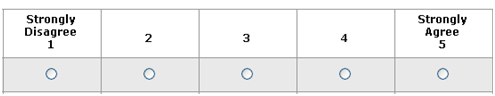
\includegraphics[width=1.0\textwidth]{img/sus-responses.png}
  \caption{Testing, 'SUS choices'} 
  \label{fig:sus_response}
\end{figure}
Because the customer was going away for two weeks and exams were approaching, this test was done before the system was finished . This affected the test results.

These are the results from the system usability test with the customer:
\begin{enumerate} \setlength{\itemsep}{0cm}\setlength{\parskip}{0cm}
	\item I think that I would like to use this system frequently. \hfill 3 
	\item I found the system unnecessarily complex. \hfill 2
	\item I thought the system was easy to use. \hfill 4
	\item I think that I would need the support of a technical person to be able to use this system.\hfill 2
	\item I found the various functions in this system were well integrated.\hfill 3
	\item I thought there was too much inconsistency in this system.\hfill 2
	\item I imagine that most people would learn to use this system very quickly.\hfill 2
	\item I found the system very cumbersome to use.\hfill 3
	\item I felt very confident using the system.\hfill 3
	\item I needed to learn a lot of things before I could get going with this system.\hfill 3
\end{enumerate}
Comments about the system: In the expert interface an error message should be shown instead of the program crashing.\\ 
A SUS score of 57.5\\

In addition, tests on three fellow students were done after the system was finished:

\begin{enumerate} \setlength{\itemsep}{0cm}\setlength{\parskip}{0cm}
	\item I think that I would like to use this system frequently. \hfill 4
	\item I found the system unnecessarily complex. \hfill 1
	\item I thought the system was easy to use. \hfill 3
	\item I think that I would need the support of a technical person to be able to use this system.\hfill 3
	\item I found the various functions in this system were well integrated.\hfill 4
	\item I thought there was too much inconsistency in this system.\hfill 1
	\item I imagine that most people would learn to use this system very quickly.\hfill 5
	\item I found the system very cumbersome to use.\hfill 2
	\item I felt very confident using the system.\hfill 3
	\item I needed to learn a lot of things before I could get going with this system.\hfill 5
\end{enumerate}

Comments about the system: Hard to see the active player when there is lots of panic on the map. Difficult to read the text in the expert interface view.\\
A SUS score of 67.5\\

\begin{enumerate} \setlength{\itemsep}{0cm}\setlength{\parskip}{0cm}
	\item I think that I would like to use this system frequently. \hfill 5 
	\item I found the system unnecessarily complex. \hfill 2
	\item I thought the system was easy to use. \hfill 4
	\item I think that I would need the support of a technical person to be able to use this system.\hfill 4
	\item I found the various functions in this system were well integrated.\hfill 5
	\item I thought there was too much inconsistency in this system.\hfill 1
	\item I imagine that most people would learn to use this system very quickly.\hfill 4
	\item I found the system very cumbersome to use.\hfill 2
	\item I felt very confident using the system.\hfill 3
	\item I needed to learn a lot of things before I could get going with this system.\hfill 4
\end{enumerate}

Comments about the system: Need to learn the game itself more than the program.\\
A SUS score of 70.\\

\begin{enumerate} \setlength{\itemsep}{0cm}\setlength{\parskip}{0cm}
	\item I think that I would like to use this system frequently. \hfill 4
	\item I found the system unnecessarily complex. \hfill 2
	\item I thought the system was easy to use. \hfill 4
	\item I think that I would need the support of a technical person to be able to use this system.\hfill 4
	\item I found the various functions in this system were well integrated.\hfill 4
	\item I thought there was too much inconsistency in this system.\hfill 2
	\item I imagine that most people would learn to use this system very quickly.\hfill 5
	\item I found the system very cumbersome to use.\hfill 1
	\item I felt very confident using the system.\hfill 3
	\item I needed to learn a lot of things before I could get going with this system.\hfill 3
\end{enumerate}

Comments about the system: A bit problematic too see the active player when the map was mostly red.\\
A SUS score of 70.\\

Because the system was not completed when we tested it with the customer, that SUS score will not be computed in the average SUS score. Therefore the average SUS score for the system is 69.1666666667, that is considered as above the average which is 68. Some of the negative scores in these tests relates to the game itself and not the system. If people that knew the game would test the system, better scores would probably occur. Therefore more time should be spent explaining the game rules before the tests. In addition most users will only use the "Play" part of the system. The "Expert Interface", "Game Master" and "Replay" parts are for the experts only, to set up, control and review games. In the SUS test, all parts of the system was tested, and that will not be the case of a regular user.\\
\\
Because it is a serious game for learning purposes, the people who are going to play the game will most likely get proper introduction to the game rules. Therefore the group are deeply satisfied with the usability of the system. 
\subsection{White Box}
For the white box testing we have done small tests locally without pushing it to git. We have tried to keep one branch on our git repository free from errors, and only pushing working and error free versions of the game. The white box testing process has been an continuously task throughout the game development. The line "console.log('error');" has of course been of great help. The testing we have done of white box  has not been documented, as we found nothing of importance to document when we decided to not use unit tests. Since this is a smaller project, members of the group has had widespread and deep knowledge of the complete source code, and therefore white box testing has been possible.


\subsection{Tests}


%%%%%%%%%%%%%%%%%%%%%%%%%%%%%%%%%%%%%%%%
% 1


{\footnotesize
\begin{table}[H]
\begin{tabular}{| p{5cm} | p{10cm} |}\hline
	\textbf{ID}	& \textbf{01}\\ \hline
	Name		& Game Start\\ \hline
	Time schedule	& Approximately 10 minutes \\ \hline
	Enviorment requirements 
		& The test computer must have internet access. \\
		& Regarding software, only a web browser is required. \\ \hline
	Test risk analasys 
		& Connection failure - Plausible \\ 
		& \emph{* Try to connect again. If the error persists, use another computer.} \\
		& \emph{* If switching computer does not resolve the connection failure, use another network.}\\ \hline
	Goal	& The test is to verify that the player can log in and start a game without problems. \\ \hline
	Actors	& Player, Game Board, \emph{Game Session, Server}\\ \hline
	Test requirements
		& The player can connect with the server. \\
		& The player can not log in with incorrect credentials. \\
		& The player can join the selected game. \\
		& The player cannot join an unintended game.\\ \hline
	End requirements 
		& The player cannot connect with the server. \\
		& The player can log in with incorrect credentials. \\
		& The player cannot join the selected game. \\
		& The player can join an unintended game. \\
		& The player disconnects. \\ \hline
	Disruption criteria 
		& The player tries to connect with the server. \\
		& The player logs in with his credentials. \\
		& The player tries to join a game. \\ \hline
	Test case
		& The player tries to connect with the server. \\
		& The player logs in with his credentials. \\
		& The player tries to join a game. \\ \hline
	Alternative case
		& The player logs in with incorrect credentials.\\
		& The player tries to join an unintended game. \\ \hline
	Test results 
		& Success \\ \hline
	Test comments
		& In order to connect to the database we have used, it is required to be connected to 
			Eduroam, or to use NTNU's VPN service\\ \hline
	Improvements needed
		& None \\ \hline
\end{tabular}


\caption{Black Box Test: Game Start}
\label{fig:black_box_test_1}
\end{table}}

%%%%%%%%%%%%%%%%%%%%%%%%%%%%%%%%%%%%%%%%
% 2

{\footnotesize
\begin{table}[H]
\begin{tabular}{| p{5cm} | p{10cm} |}\hline
	\textbf{ID}	& \textbf{02}\\ \hline
	Name		& Gamepad Interaction\\ \hline
	Time schedule	& Approximately 10 minutes\\ \hline
	Enviorment requirements 
		& The test computer must have internet access. \\
		& Regarding software, only a web browser is required. \\ \hline
	Test risk analasys 
		& Connection failure - Plausible \\
		& \emph{* Try to connect again. If the error persists, use another computer.} \\
		& \emph{* If switching computer does not resolve the connection failure, use another network.}\\ 
		& Hardware fault - unlikely \\
		& \emph{* Use another computer within the group.} \\ \hline
	Goal	& The test is to verify that the gamepad is usable with the game and to the team’s satisfaction. \\ \hline
	Actors	& Player, Game Board, \emph{Game Session, Server}\\ \hline
	Test requirements
		& An expert has created a game. \\
		& The player is inside a game session. \\ \hline
	End requirements 
		& The gamepad works with every part of the game.\\ \hline
	Disruption criteria 
		& The gamepad cannot move or interact with the game board. \\
		& The gamepad can pick up objects but not hold on to them. \\
		& The gamepad cannot move the objects to another point. \\
		& The player disconnects. \\ 
		& Unexpected faults with the gamepad. \\ \hline
	Test case
		& The player checks the gamepad for interaction possibilities with the game board. \\
		& The player then checks if the gamepad can move objects around with the gamepad. \\
		& The player verifies that the gamepad can move objects to another location. \\ \hline
	Alternative case
		& \emph{None}\\ \hline
	Test results 
		& Success\\ \hline
	Test comments
		& All the buttons and drag events are functional\\ \hline
	Improvements needed
		& Making it more visible what parts can be used/dragged \\ \hline
\end{tabular}


\caption{Black Box Test: Gamepad interaction}
\label{fig:black_box_test_2}
\end{table}}

%%%%%%%%%%%%%%%%%%%%%%%%%%%%%%%%%%%%%%%%
% 3

{\footnotesize
\begin{table}[H]
\begin{tabular}{| p{5cm} | p{10cm} |}\hline
	\textbf{ID}	& \textbf{03}\\ \hline
	Name		& Game art.\\ \hline
	Time schedule	& Approximately 10 minutes.\\ \hline
	Enviorment requirements 
		& The test computer must have internet access. \\
		& Regarding software, only a web browser is required. \\ \hline
	Test risk analasys 
		& Connection failure - Plausible \\
		& \emph{* Try to connect again. If the error persists, use another computer.}\\
		& \emph{* If switching computer does not resolve the connection failure, use another network.}\\ 
		& Hardware fault - unlikely \\
		& \emph{* Use another computer within the group.} \\ \hline
	Goal	& The test is to verify that the game art is according to the standards and has no deviations. \\ \hline
	Actors	& Player, Game Board, \emph{Game Session, Server}\\ \hline
	Test requirements
		& An expert has created a game.\\
		& The player is inside a game session.\\ \hline
	End requirements 
		& The board model has no deviations (fragments, overlappings, clippings, out of frame, correct colors and form). \\
		& The player models are as they should be (correct colors, png, way and position). \\
		& Other object models (blockade and information center) are satisfiable. \\ \hline
	Disruption criteria 
		& The board model has one of the mentioned deviations or other impurities.\\
		& The player model has one deviation or an unexpected fault.\\
		& Other object models have faults or deviations.\\
		& The player cannot move or place the intended objects on the board.\\
		& The player disconnects \\ \hline
	Test case
		& The player checks the board thoroughly for deviations from the planned model.\\
		& The player then checks the player model for impurities, also while the model is moving.\\
		& The player checks the other game pieces, information center and blockades, 
			while they are being placed on the board or moving.\\ \hline
	Alternative case
		& \emph{None}\\ \hline
	Test results 
		& Success \\ \hline
	Test comments
		& Everything looks as intended, without diviations. \\ \hline
	Improvements needed
		& We are not designers, so it could probably be more visually appealing \\ \hline
\end{tabular}


\caption{Black Box Test: Game art}
\label{fig:black_box_test_3}
\end{table}}

%%%%%%%%%%%%%%%%%%%%%%%%%%%%%%%%%%%%%%%%
% 4

{\footnotesize
\begin{table}[H]
\begin{tabular}{| p{5cm} | p{10cm} |}\hline
	\textbf{ID}	& \textbf{04}\\ \hline
	Name		& Game Movement\\ \hline
	Time schedule	& Approximately 10 minutes.\\ \hline
	Enviorment requirements 
		& The test computer must have internet access. \\
		& Regarding software, only a web browser is required. \\ \hline
	Test risk analasys 
		& Connection failure - Plausible \\ 
		& \emph{* Try to connect again. If the error persists, use another computer.}\\
		& \emph{* If switching computer does not resolve the connection failure, use another network.}\\ 
		& Hardware fault - unlikely \\
		& \emph{* Use another computer within the group.} \\ \hline
	Goal	& The test is to verify that the game movements are functional and according to the standards.\\ \hline
	Actors	& Player, Game Board, \emph{Game Session, Server}\\ \hline
	Test requirements
		& An expert has created a game. \\
		& The player is inside a game session. \\ \hline
	End requirements 
		& The movement of the player model is satisfiable.\\
		& The placement of the information center model is satisfiable.\\
		& The placement of the blockade model is satisfiable.\\
		& The movement of the information cards is satisfiable. \\ \hline
	Disruption criteria 
		& The movement of one of the objects is glitchy, flickering, moving out of bounce 
			or something unexpected happens while the player is moving one of the objects. \\
		& The player cannot see the object after it is moved. \\
		& The object appears in the wrong place after it is moved or placed on the board. \\
		& The player cannot locate the object intended to move. \\
		& The player loses the object without human fault, while holding it in the “drag and drop”. \\
		& The player cannot move or place intended objects on the board. \\
		& The player disconnects. \\ \hline
	Test case
		& The player checks the player model while in movement and after it is dropped on the board.\\
		& The player checks the information cards after and while they are in movement.\\
		& The player checks the placement of the blockades.\\ 
		& The player checks the placements of the information center. \\ \hline
	Alternative case
		& \emph{None}\\ \hline
	Test results 
		& \\ \hline
	Test comments
		& \\ \hline
	Improvements needed
		& \\ \hline
\end{tabular}


\caption{Black Box Test: Game movement}
\label{fig:black_box_test_4}
\end{table}}


%%%%%%%%%%%%%%%%%%%%%%%%%%%%%%%%%%%%%%%%
% 5

{\footnotesize
\begin{table}[H]
\begin{tabular}{| p{5cm} | p{10cm} |}\hline
	\textbf{ID}	& \textbf{05} \\ \hline
	Name		& Game flow\\ \hline
	Time schedule	& Approximately 10 minutes.\\ \hline
	Enviorment requirements 
		& The test computer must have internet access. \\
		& Regarding software, only a web browser is required. \\ \hline
	Test risk analasys 
		& Connection failure - Plausible \\
		& \emph{* Try to connect again. If the error persists, use another computer.} \\
		& \emph{* If switching computer does not resolve the connection failure, use another network.}\\ 
		& Hardware fault - unlikely \\
		& \emph{* Use another computer within the group.} \\ \hline
	Goal	& The test is to verify that the game handles turns correctly. \\ \hline
	Actors	& Player, Game Board, \emph{Game Session, Server} \\ \hline
	Test requirements
		& An expert has created a game.\\
		& The player is inside a game session.\\ \hline
	End requirements 
		& The game turns work as they were intended. \\
		& Turns do not change before the player gives the command. \\
		& The player is able to use his or her complete turn, use the right amount of actions within a turn.\\ \hline
	Disruption criteria 
		& The game turn changes before the command is given. \\
		& The game turn does not change when the command is given. \\
		& The player is unable to use his or her complete turn, missing actions. \\
		& The current player does not change, or the previous player can still move its player model. \\
		& The player is able to use more than the given actions. \\
		& An unexpected deviation occurs.  \\
		& The player disconnects. \\ \hline
	Test case
		& The player uses the the intended actions within its turn. \\
		& The player gives the command to change game turn. \\ \hline
	Alternative case
		& The player tries to use more actions than there are in a game turn. \\
		& The player tries to move the previous player model. \\ \hline
	Test results 
		& \\ \hline
	Test comments
		& \\ \hline
	Improvements needed
		& \\ \hline
\end{tabular}


\caption{Black Box Test: Game flow}
\label{fig:black_box_test_5}
\end{table}}

%%%%%%%%%%%%%%%%%%%%%%%%%%%%%%%%%%%%%%%%
% 6

{\footnotesize
\begin{table}[H]
\begin{tabular}{| p{5cm} | p{10cm} |}\hline
	\textbf{ID}	& \textbf{06} \\ \hline
	Name		& Game events\\ \hline
	Time schedule	& Approximately 10 minutes\\ \hline
	Enviorment requirements 
		& The test computer must have internet access. \\
		& Regarding software, only a web browser is required. \\ \hline
	Test risk analasys 
		& Connection failure - Plausible \\
		& \emph{* Try to connect again. If the error persists, use another computer.} \\
		& \emph{* If switching computer does not resolve the connection failure, use another network.}\\ 
		& Hardware fault - unlikely \\
		& \emph{* Use another computer within the group.} \\ \hline
	Goal	& The test is to verify that the game events are as intended. \\ \hline
	Actors	& Player, Game Board, \emph{Game Session, Server}\\ \hline
	Test requirements
		& An expert has created a game. \\
		& The player is inside a game session. \\ \hline
	End requirements 
		& The game timer resets upon the right time.\\
		& The panic levels increase when the timer runs out.\\
		& The panic level in the correct zones decreases when the information cards are used.\\
		& The panic level increases in the correct zones when event cards are presented.\\
		& The panic levels decrease when people are moved out of a zone.\\
		& Effects from event cards are carried out as expected (i.e. the player must 
			skip a turn or he loses 2 actions in his next turn). \\ \hline
	Disruption criteria 
		& The game timer does not reset upon the expected time.\\
		& The panic levels do not increase when the time runs out.\\
		& The panic levels do not decrease when information card effects are used.\\
		& The panic level does not decrease when people are mowed out of a zone.\\
		& The panic levels increase or decrease in the wrong zone when an effect is applied to the game.\\
		& Effects from event cards are not recognized.\\
		& The player disconnects.\\ \hline
	Test case
		& The player checks that the timer is reset when the time runs out.\\
		& The player checks that the panic level is increased in all eligible zones when the time runs out.\\
		& The player checks that the panic levels decrease in the correct zones when an information card is used.\\
		& The player checks that the panic levels are increased in the correct zones when an event card with this effect is viewed. \\
		& The player checks if all the effects from the event cards are upheld. \\ \hline
	Alternative case
		& \emph{None}\\ \hline
	Test results 
		& \\ \hline
	Test comments
		& \\ \hline
	Improvements needed
		& \\ \hline
\end{tabular}


\caption{Black Box Test: Game events}
\label{fig:black_box_test_6}
\end{table}}

%%%%%%%%%%%%%%%%%%%%%%%%%%%%%%%%%%%%%%%%
% 7

{\footnotesize
\begin{table}[H]
\begin{tabular}{| p{5cm} | p{10cm} |}\hline
	\textbf{ID}	& \textbf{07} \\ \hline
	Name		& Testing memory overload\\ \hline
	Time schedule	& Approximately 2 hours.\\ \hline
	Enviorment requirements 
		& The test computer must have internet access. \\
		& Regarding software, only a web browser is required. \\ \hline
	Test risk analasys 
		& Connection failure - Plausible \\
		& \emph{* Try to connect again. If the error persists, use another computer.} \\
		& \emph{* If switching computer does not resolve the connection failure, use another network.}\\ 
		& Hardware fault - unlikely \\
		& \emph{* Use another computer within the group.} \\ \hline
	Goal	& The test is to verify that the game does not run out of memory and can continue for an extended period of time. \\ \hline
	Actors	& Player, Game Board, \emph{Game Session, Server} \\ \hline
	Test requirements
		& An expert has created a game.\\
		& The player is inside a game session.\\ \hline
	End requirements 
		& The game should not run out of memory.\\ \hline
	Disruption criteria 
		& The game runs out of memory. \\
		& The game freezes. \\
		& The player disconnects.\\
		& Unexpected faults with the game.\\ \hline
	Test case
		& The player(s) tries to use up as much memory as possible.\\ \hline
	Alternative case
		& \emph{None}\\ \hline
	Test results 
		& \\ \hline
	Test comments
		& \\ \hline
	Improvements needed
		& \\ \hline
\end{tabular}


\caption{Black Box Test: Memory Overload}
\label{fig:black_box_test_7}
\end{table}}


%%%%%%%%%%%%%%%%%%%%%%%%%%%%%%%%%%%%%%%%
% 8

{\footnotesize
\begin{table}[H]
\begin{tabular}{| p{5cm} | p{10cm} |}\hline
	\textbf{ID}	& \textbf{08} \\ \hline
	Name		& Multiple parallel sessions\\ \hline
	Time schedule	& Approximately 20 minutes\\ \hline
	Enviorment requirements 
		& The test computer must have internet access. \\
		& Regarding software, only a web browser is required. \\ \hline
	Test risk analasys 
		& Connection failure - Plausible \\
		& \emph{* Try to connect again. If the error persists, use another computer.} \\
		& \emph{* If switching computer does not resolve the connection failure, use another network.}\\
		& Hardware fault - unlikely \\
		& \emph{* Use another computer within the group.} \\ \hline
	Goal	& The test is to verify that the server is capable of running several game sessions at the same time \\ \hline
	Actors	& Player, Game Board, \emph{Game Session, Server} \\ \hline
	Test requirements
		& An expert has created several games.\\
		& A set of players are inside a game session.\\
		& Another set of players are in another game session. \\ \hline
	End requirements 
		& All game sessions run smoothly, and the server is able to store the separate replays.\\ \hline
	Disruption criteria 
		& One session takes control of events in another session.\\
		& The server is unable to handle the sessions, and freezes.\\
		& A game session closes unexpectedly. \\
		& The players disconnect.\\
		& Unexpected faults with the server. \\ \hline
	Test case
		& The players enter separate game sessions.\\
		& The players then begin playing the game as normal.\\
		& At predetermined times, the players perform actions at the same time in the separate sessions.\\ \hline
	Alternative case
		& \emph{None}\\ \hline
	Test results 
		& \\ \hline
	Test comments
		& \\ \hline
	Improvements needed
		& \\ \hline
\end{tabular}


\caption{Black Box Test: Parallel sessions}
\label{fig:black_box_test_8}
\end{table}}

%%%%%%%%%%%%%%%%%%%%%%%%%%%%%%%%%%%%%%%%
% 9

{\footnotesize
\begin{table}[H]
\begin{tabular}{| p{5cm} | p{10cm} |}\hline
	\textbf{ID}	& \textbf{09} \\ \hline
	Name		& Platform compatibility\\ \hline
	Time schedule	& Approximately 20 minutes.\\ \hline
	Enviorment requirements 
		& The test computer must have internet access. \\
		& Regarding software, a range of different web browsers are required.\\
		& - Internet Explorer\\
		& - Mozilla Firefox\\
		& - Google Chrome\\
		& - Safari\\
		& - Opera\\ \hline
	Test risk analasys
		& Connection failure - Plausible \\
		& \emph{* Try to connect again. If the error persists, use another computer.} \\
		& \emph{* If switching computer does not resolve the connection failure, use another network.}\\
		& Hardware fault - unlikely \\
		& \emph{* Use another computer within the group.} \\ \hline
	Goal	& The test is to verify that the game is compatible with different web browsers.\\ \hline
	Actors	& Player, Game Board, \emph{Game Session, Server}\\ \hline
	Test requirements
		& An expert has created a game.\\
		& The player is inside a game session.\\ \hline
	End requirements 
		& The game works on all platforms. \\ \hline
	Disruption criteria 
		& The game does not load in one of the web browsers. \\
		& The game only works partially in one or more browsers. \\ \hline
	Test case
		& The player checks if the game can be loaded in all web browsers.\\
		& The player goes through use cases 6 and 7 to check for functionality with all web browsers.\\ \hline
	Alternative case
		& \emph{None}\\ \hline
	Test results 
		& \\ \hline
	Test comments
		& \\ \hline
	Improvements needed
		& \\ \hline
\end{tabular}

\caption{Black Box Test: Game Start}
\label{fig:black_box_test_9}
\end{table}}












\subsection{Usability tests}
%%%%%%%%%%%%%%%%%%%%%%%%%%%%%%%%%%%%%%%%
% 1

{\footnotesize
\begin{table}[H]
\begin{tabular}{| p{5cm} | p{10cm} |}\hline
	\textbf{ID}	& \textbf{01} \\ \hline
	Name		& Player logging in\\ \hline
	Corresponding usecase & ID 1\\ \hline
	Time schedule	& Approximately 10 minutes\\ \hline
	Enviorment requirements 
		& The test computer must have internet access. \\ \hline
	Test risk analasys 
		& Connection failure - Plausible \\
		& \emph{* Try to connect again. If the error persists, use another computer.} \\
		& \emph{* If switching computer does not resolve the connection failure, use another network.}\\
		& Hardware fault - unlikely \\
		& \emph{* Use another computer within the group.} \\
		& The test person has to leave - unlikely \\
		& \emph{* Schedule a sufficient time slot beforehand.} \\
		& \emph{* If that proves too difficult, schedule a new meeting.}\\ \hline
	Actors	& Player, \emph{Server}\\ \hline
	Test requirements & As described in Use Case 01 \\ \hline
	Disruption criteria & As described in Use Case 01  \\ \hline
	Test results & Could not log in.\\ \hline
	Test comments & The implementation of users was not prioritized, and is unfinished. \\ \hline
	Improvements needed & \\ \hline
\end{tabular}


\caption{Usability Test: Player logging in}
\label{fig:usability_test_1}
\end{table}}

%%%%%%%%%%%%%%%%%%%%%%%%%%%%%%%%%%%%%%%%
% 2

{\footnotesize
\begin{table}[H]
\begin{tabular}{| p{5cm} | p{10cm} |}\hline
	\textbf{ID}	& \textbf{02} \\ \hline
	Name		& Expert logging in\\ \hline
	Corresponding usecase & ID 2\\ \hline
	Time schedule	& Approximately 10 minutes\\ \hline
	Enviorment requirements 
		& The test computer must have internet access. \\ \hline
	Test risk analasys 
		& Connection failure - Plausible \\
		& \emph{* Try to connect again. If the error persists, use another computer.} \\
		& \emph{* If switching computer does not resolve the connection failure, use another network.}\\
		& Hardware fault - unlikely \\
		& \emph{* Use another computer within the group.} \\
		& The test person has to leave - unlikely \\
		& \emph{* Schedule a sufficient time slot beforehand.} \\
		& \emph{* If that proves too difficult, schedule a new meeting.}\\ \hline
	Actors	& Expert, \emph{Server}\\ \hline
	Test requirements & As described in Use Case 02 \\ \hline
	Disruption criteria & As described in Use Case 02  \\ \hline
	Test results & Could not log in. \\ \hline
	Test comments & The implementation of an administrator user was not prioritized, and is unfinished.\\ \hline
	Improvements needed & \\ \hline
\end{tabular}


\caption{Usability Test: Expert logging in}
\label{fig:usability_test_2}
\end{table}}

%%%%%%%%%%%%%%%%%%%%%%%%%%%%%%%%%%%%%%%%
% 3

{\footnotesize
\begin{table}[H]
\begin{tabular}{| p{5cm} | p{10cm} |}\hline
	\textbf{ID}	& \textbf{03} \\ \hline
	Name		& Game Setup\\ \hline
	Corresponding usecase & ID 3\\ \hline
	Time schedule	& Approximately 10 minutes\\ \hline
	Enviorment requirements 
		& The test computer must have internet access. \\
		& The expert is logged in\\ \hline
	Test risk analasys 
		& Connection failure - Plausible \\
		& \emph{* Try to connect again. If the error persists, use another computer.} \\
		& \emph{* If switching computer does not resolve the connection failure, use another network.}\\
		& Hardware fault - unlikely \\
		& \emph{* Use another computer within the group.} \\
		& The test person has to leave - unlikely \\
		& \emph{* Schedule a sufficient time slot beforehand.} \\
		& \emph{* If that proves too difficult, schedule a new meeting.}\\ \hline
	Actors	& Expert, \emph{Server}\\ \hline
	Test requirements & As described in Use Case 03 \\ \hline
	Disruption criteria & As described in Use Case 03  \\ \hline
	Test results & Successfully made a game template.
		\\ \hline
	Test comments & Difficult for a first time user to know how to set up the game.
		\\ \hline
	Improvements needed & Add descriptions on how to use the different features as well as make the shortcuts visible. 
		\\ \hline
\end{tabular}


\caption{Usability Test: Game setup}
\label{fig:usability_test_3}
\end{table}}


%%%%%%%%%%%%%%%%%%%%%%%%%%%%%%%%%%%%%%%%
% 4

{\footnotesize
\begin{table}[H]
\begin{tabular}{| p{5cm} | p{10cm} |}\hline
	\textbf{ID}	& \textbf{04} \\ \hline
	Name		& Watcher \\ \hline
	Corresponding usecase & ID 4\\ \hline
	Time schedule	& Approximately 10 minutes\\ \hline
	Enviorment requirements 
		& The test computer must have internet access. \\ 
		& The expert is logged in\\ \hline
	Test risk analasys 
		& Connection failure - Plausible \\
		& \emph{* Try to connect again. If the error persists, use another computer.} \\
		& \emph{* If switching computer does not resolve the connection failure, use another network.}\\
		& Hardware fault - unlikely \\
		& \emph{* Use another computer within the group.} \\
		& The test person has to leave - unlikely \\
		& \emph{* Schedule a sufficient time slot beforehand.} \\
		& \emph{* If that proves too difficult, schedule a new meeting.}\\ \hline
	Actors	& Expert, \emph{Server}\\ \hline
	Test requirements & As described in Use Case 04 \\ \hline
	Disruption criteria & As described in Use Case 04  \\ \hline
	Test results & Successfully joined a game session and watched the game. \\ \hline
	Test comments & \\ \hline
	Improvements needed & \\ \hline
\end{tabular}


\caption{Usability Test: Watcher}
\label{fig:usability_test_4}
\end{table}}


%%%%%%%%%%%%%%%%%%%%%%%%%%%%%%%%%%%%%%%%
% 5

{\footnotesize
\begin{table}[H]
\begin{tabular}{| p{5cm} | p{10cm} |}\hline
	\textbf{ID}	& \textbf{05} \\ \hline
	Name		& Join Game\\ \hline
	Corresponding usecase & ID 5\\ \hline
	Time schedule	& Approximately 10 minutes\\ \hline
	Enviorment requirements 
		& The test computer must have internet access. \\ 
		& The expert has created a game session\\ \hline
	Test risk analasys 
		& Connection failure - Plausible \\
		& \emph{* Try to connect again. If the error persists, use another computer.} \\
		& \emph{* If switching computer does not resolve the connection failure, use another network.}\\
		& Hardware fault - unlikely \\
		& \emph{* Use another computer within the group.} \\
		& The test person has to leave - unlikely \\
		& \emph{* Schedule a sufficient time slot beforehand.} \\
		& \emph{* If that proves too difficult, schedule a new meeting.}\\ \hline
	Actors	& Player, \emph{Game Session, Server}\\ \hline
	Test requirements & As described in Use Case 05 \\ \hline
	Disruption criteria & As described in Use Case 05  \\ \hline
	Test results & Successfully joined a game. \\ \hline
	Test comments & none \\ \hline
	Improvements needed & none \\ \hline
\end{tabular}


\caption{Usability Test: Join Game}
\label{fig:usability_test_5}
\end{table}}


%%%%%%%%%%%%%%%%%%%%%%%%%%%%%%%%%%%%%%%%
% 6

{\footnotesize
\begin{table}[H]
\begin{tabular}{| p{5cm} | p{10cm} |}\hline
	\textbf{ID}	& \textbf{06} \\ \hline
	Name		& Move game pieces\\ \hline
	Corresponding usecase & ID 6\\ \hline
	Time schedule	& Approximately 10 minutes\\ \hline
	Enviorment requirements 
		& The test computer must have internet access. \\ 
		& The player has joined the game\\ \hline
	Test risk analasys 
		& Connection failure - Plausible \\
		& \emph{* Try to connect again. If the error persists, use another computer.} \\
		& \emph{* If switching computer does not resolve the connection failure, use another network.}\\
		& Hardware fault - unlikely \\
		& \emph{* Use another computer within the group.} \\
		& The test person has to leave - unlikely \\
		& \emph{* Schedule a sufficient time slot beforehand.} \\
		& \emph{* If that proves too difficult, schedule a new meeting.}\\ \hline
	Actors	& Player, Game board, \emph{Game session, Server}\\ \hline
	Test requirements & As described in Use Case 06 \\ \hline
	Disruption criteria & As described in Use Case 06  \\ \hline
	Test results & Successfully moved game pieces. \\ \hline
	Test comments & The game movements were all accordingly to the game rules \\ \hline
	Improvements needed & none \\ \hline
\end{tabular}


\caption{Usability Test: Move game pieces}
\label{fig:usability_test_6}
\end{table}}

%%%%%%%%%%%%%%%%%%%%%%%%%%%%%%%%%%%%%%%%
% 7

{\footnotesize
\begin{table}[H]
\begin{tabular}{| p{5cm} | p{10cm} |}\hline
	\textbf{ID}	& \textbf{07} \\ \hline
	Name		& Use information cards\\ \hline
	Corresponding usecase & ID 7\\ \hline
	Time schedule	& Approximately 10 minutes\\ \hline
	Enviorment requirements 
		& The test computer must have internet access. \\ 
		& The player is ingame, and has information cards.\\ \hline
	Test risk analasys 
		& Connection failure - Plausible \\
		& \emph{* Try to connect again. If the error persists, use another computer.} \\
		& \emph{* If switching computer does not resolve the connection failure, use another network.}\\
		& Hardware fault - unlikely \\
		& \emph{* Use another computer within the group.} \\
		& The test person has to leave - unlikely \\
		& \emph{* Schedule a sufficient time slot beforehand.} \\
		& \emph{* If that proves too difficult, schedule a new meeting.}\\ \hline
	Actors	& Player, Game Board, \emph{Game session, Server}\\ \hline
	Test requirements & As described in Use Case 07 \\ \hline
	Disruption criteria & As described in Use Case 07  \\ \hline
	Test results & Successfully used information cards \\ \hline
	Test comments & The effects of the information cards was done properly. \\ \hline
	Improvements needed & none \\ \hline
\end{tabular}


\caption{Usability Test: Use information cards}
\label{fig:usability_test_7}
\end{table}}

%%%%%%%%%%%%%%%%%%%%%%%%%%%%%%%%%%%%%%%%
% 8

{\footnotesize
\begin{table}[H]
\begin{tabular}{| p{5cm} | p{10cm} |}\hline
	\textbf{ID}	& \textbf{08} \\ \hline
	Name		& Use player action\\ \hline
	Corresponding usecase & ID 8\\ \hline
	Time schedule	& Approximately 10 minutes\\ \hline
	Enviorment requirements 
		& The test computer must have internet access. \\ 
		& The player is ingame\\ \hline
	Test risk analasys 
		& Connection failure - Plausible \\
		& \emph{* Try to connect again. If the error persists, use another computer.} \\
		& \emph{* If switching computer does not resolve the connection failure, use another network.}\\
		& Hardware fault - unlikely \\
		& \emph{* Use another computer within the group.} \\
		& The test person has to leave - unlikely \\
		& \emph{* Schedule a sufficient time slot beforehand.} \\
		& \emph{* If that proves too difficult, schedule a new meeting.}\\ \hline
	Actors	& Player, Game Board, \emph{Game session, Server}\\ \hline
	Test requirements & As described in Use Case 08 \\ \hline
	Disruption criteria & As described in Use Case 08  \\ \hline
	Test results & All different user actions was successfully used. \\ \hline
	Test comments & Add and remove roadblock/information center, decrease panic and move people all worked accordingly to the game rules. \\ \hline
	Improvements needed & none \\ \hline
\end{tabular}


\caption{Usability Test: Use player action}
\label{fig:usability_test_8}
\end{table}}








